\section{Introduction}
In this analysis a search for a new particle decaying into a $t\bar{t}$ pair is done using data collected by the ATLAS experiment at the Large Hadron Collider (LHC) at CERN. Such a particle could be associated with a resonance predicted by an expansion of the Standard Model of particle physics (SM).

\section{Theoretic Foundations}

\begin{figure}[tb]
  \centering
  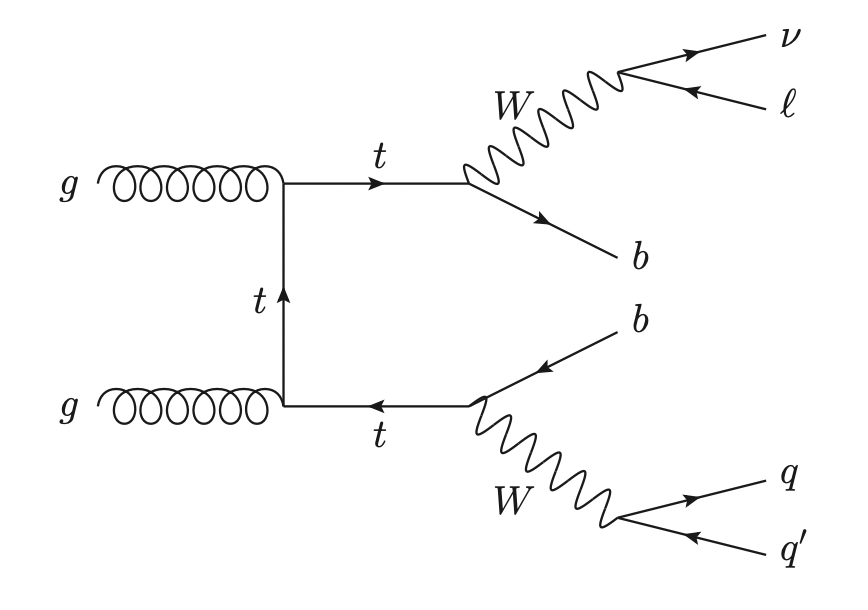
\includegraphics[width=.8\textwidth]{graphics/top_decay.png}
  \caption{Example of a leading order Feynman diagram for top quark production and decay in $pp$ collisions. The $t\bar{t}$ pair is produced via gluon-gluon fusion and decays in the \textit{lepton+jets} channel.~\cite{anleitung}}
  \label{fig:decay}
\end{figure}

The top quark is the heaviest elementary particle in the SM with a mass of $\SI{173}{\giga\eV}$~\cite{pdg} and a corrispondingly short lifetime of approximately $\SI{5e-25}{\s}$. Therefore it does not behave like other quarks, as it does not hadronise before decaying, offering a unique research sector in particle physics.
In \autoref{fig:decay} a leading order feynman diagram of top quark production and decay is shown to visualise the process.
It is dominantly produced in a $t\bar{t}$ pair via the strong interaction, e.g. via gluon gluon fusion in $pp$ collisions. The top quark decays almost exclusively via the weak interaction into a $W^+$ boson and a $b$ quark, but also a $s$ or $d$ quark is possible, though rarely observed.
The $W^+$ boson can either decay into into a lepton and its correspondig neutrino $W^+ \to \ell^+ \nu_\ell$, where $\ell \in \{e, \mu, \tau\}$, or into a quark and an anti-quark $W^+ \to q\bar{q}\prime$, where $q \in \{u, c\}$ and $\bar{q}\prime \in \{\bar{d}, \bar{s}\}$.
The quark hadronises, reulting in a colour neutral jet. The channel in which both $W$ bosons decay into leptons and neutrinos is called the \textit{dilepton channel}, whereas the channel in which both decay into quarks is called the \textit{all-hadronic} channel. If one $W$ boson decays into leptons and the other one into quarks it is called the \textit{lepton+jets} channel.

\section{The ATLAS detector}

\begin{figure}[tb]
  \centering
  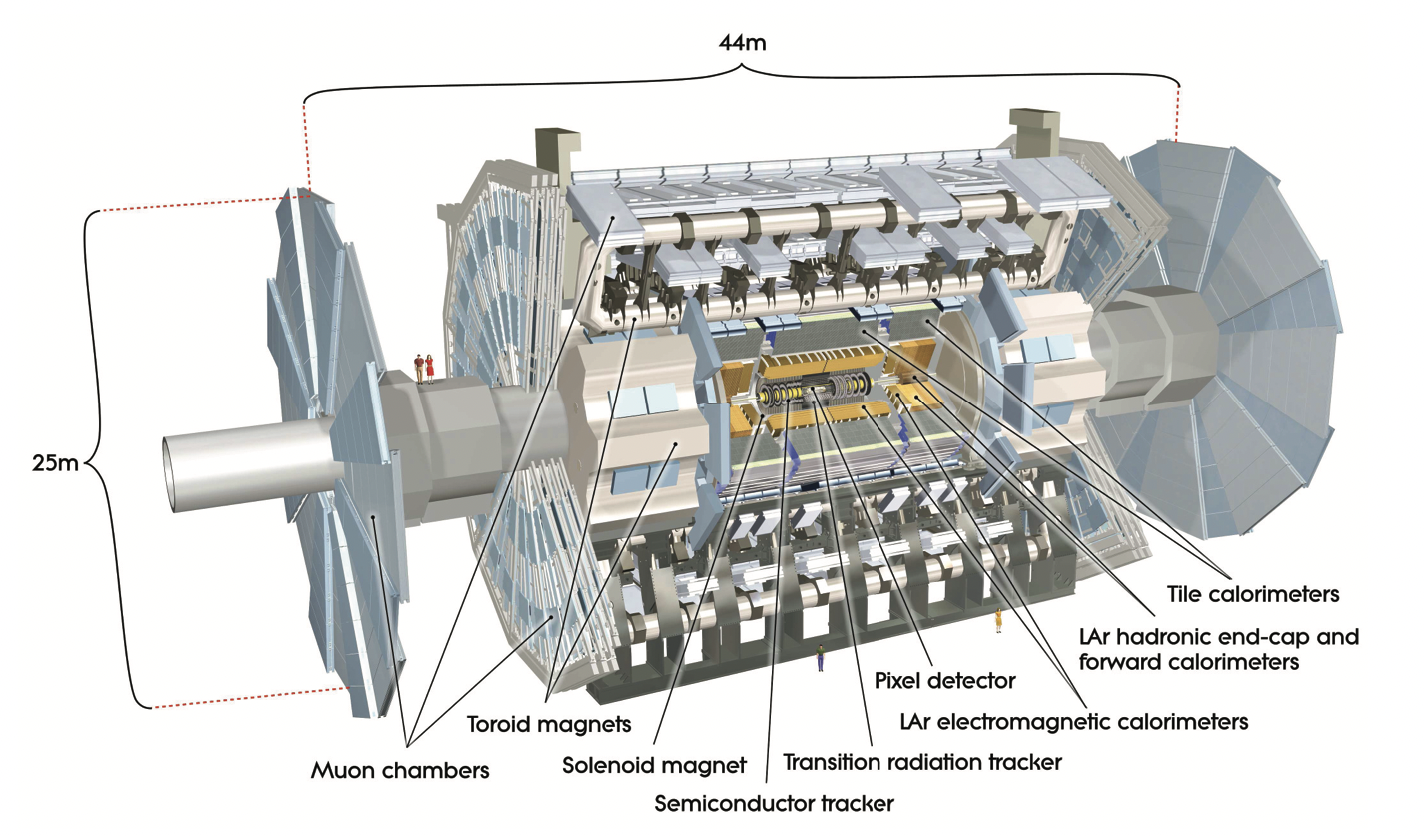
\includegraphics[width=.8\textwidth]{graphics/detector.png}
  \caption{Sketch of the ATLAS detector. \cite{ATLAS}}
  \label{fig:detector}
\end{figure}

The data analysed in this analysis was collected by the ATLAS experiment~\cite{ATLAS} at the LHC~\cite{LHC} at CERN. The detector is depicted in \autoref{fig:detector}. It is designed to be a general-purpose detector, ensuring that the detector is able to detect almost any form of ocurring new physics. The detector can be divided into four major systems: the inner detector, the calorimeters, the muon spectrometer and the magnet system.

The inner detector is the part of the detector nearest to the interaction point. It consists of a silicon pixel detector, followed by the semi-conductor tracker, which is a silicon strip detector, and the transition radiation tracker (TRT), which is a combination od a straw traker and a transition radiation tracker. The inner detector is used to measure the tracks of charged particles inside the detector. The pixel detector has a resolution high enough to identify displaced secondary vertices, which is important for identification of $b$-jets for example. The TRT also offers the ability to identify electrons and positrons. Due to their low mass they can reach higher velocities resulting in a larger amount of emitted transition radiation.

The inner detector is followed by the calorimeters. This is the only detector component able to detect neutral particles.
The LAr calorimeter is an electromagnetic sampling calorimeter with liquid argon as sampling material. For enhanced resolution it has an accordion-like structure. The LAr calorimeter is used to measure the energy of electrons, positrons and photons that deposit all of their energy in the calorimeter.
Afterwards surviving particles arrive the tile calorimeter which is a hadronic calorimeter. It works the same as the LAr calorimeter, but optimised to measure the deposited energy of hadronic showers.

The outermost system is the muon spectrometer, since muons are observed as minimum ionising particles in $pp$ collisions and are therefore able to travel through the whole detector. The muon spectrometer is used to measure tracks of those muons, additionally to those recorded by the inner detector.

The inner detector is surrounded by a solenoid magnet. The magnetic field inside the inner detector causes charged particles to drift. From the resulting curvature of the tracks a particle's momentum can be inferred.
Similarly, a toroid magnet generates a magnetic field in the muon chambers, allowing to infer muon momenta the same way.
